\documentclass{article}
% translate with >> pdflatex -shell-escape <file>

% This file is an extract of the PGFPLOTS manual, copyright by Christian Feuersaenger.
% 
% Feel free to use it as long as you cite the pgfplots manual properly.
%
% See
%   http://pgfplots.sourceforge.net/pgfplots.pdf
% for the complete manual.
%
% Any required input files (for <plot table> or <plot file> or the table package) can be downloaded
% at
% http://www.ctan.org/tex-archive/graphics/pgf/contrib/pgfplots/doc/latex/
% and
% http://www.ctan.org/tex-archive/graphics/pgf/contrib/pgfplots/doc/latex/plotdata/

\usepackage{pgfplots}
\pgfplotsset{compat=newest}

\pagestyle{empty}

\begin{document}
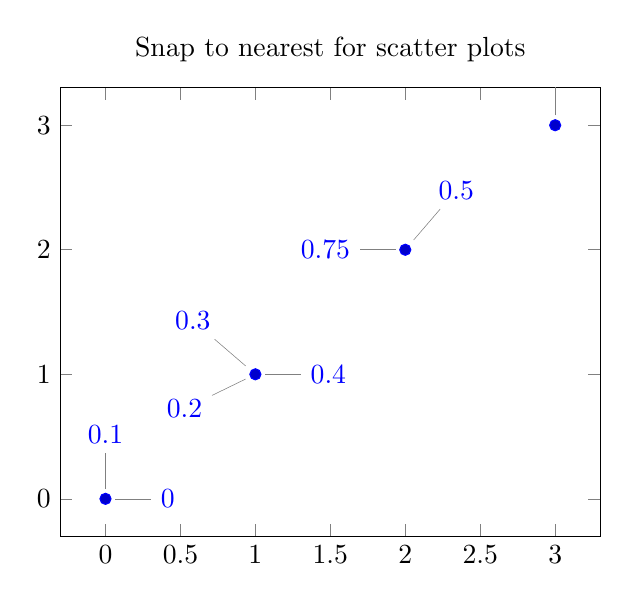
\begin{tikzpicture}
\begin{axis}[title=Snap to nearest for scatter plots]
\addplot+[only marks] 
	coordinates {(0,0) (1,1) (2,2) (3,3)} 
	node[pos=0,   pin=0  :0   ] {}
	node[pos=0.1, pin=90 :0.1 ] {}
	node[pos=0.2, pin=200:0.2 ] {}
	node[pos=0.3, pin=135:0.3 ] {}
	node[pos=0.4, pin=0  :0.4 ] {}
	node[pos=0.5, pin=60 :0.5 ] {}
	node[pos=0.75,pin=180:0.75] {}
	node[pos=1,   pin=90 :1   ] {}
;
\end{axis}
\end{tikzpicture}
\end{document}
